% Chapter IV
\makeatletter
\def\input@path{{../}}
\makeatother
\documentclass[../main.tex]{subfiles}
\begin{document}
\chapter{Cloud voids - interpretation and explanation} % Chapter title

\label{ch:holes} % For referencing the chapter elsewhere, use \autoref{ch:name} 

%----------------------------------------------------------------------------------------
\section{Cloud voids experiment results}
Cloud voids observations were performed at UFS on Zugspitze slopes in August 2011. Experimental methods used were described in Sec.\autoref{ch2s4}. This section presents the measurement results.\\
First, 30-minute long records of turbulence and droplet properties corresponding to the camera acquisition series in two mesurement days were chosen for analysis. Droplet size raw measurements are presented in Fig. \ref{fig:ch4_1} and the corresponsing statistics in Table \ref{tab:ch4_1}. Both cloud droplets, as well as drizzle drops were captured. Next, the probability distribution of the droplet size has been calculated and presented in Fig.\ref{fig:ch4_2}. For comparison, the corresponding gaussian distributions have been plotted. It clearly shows that the actual distributions are far from gaussian. There are clear differences between the distributions measured on both days: the first one is much wider, the tail reach larger values and on average the droplets are about twice as big.

\begin{figure}[h]
\centering
\noindent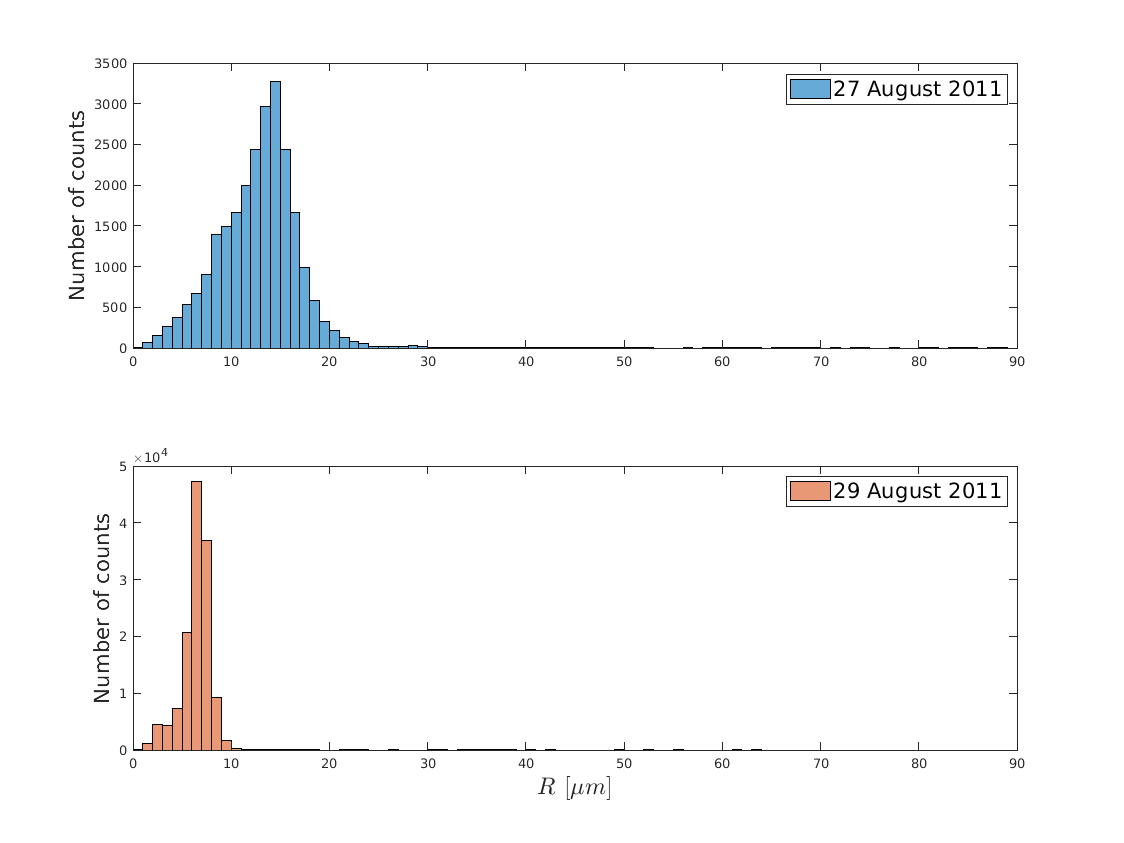
\includegraphics[width=30pc]{Hist_counts_raw.png}
\caption{Histograms of droplet size counts measured with a PDI probe at the UFS on 27th and 29th of August 2011.}
\label{fig:ch4_1}
\end{figure}

\begin{figure}[h]
\centering
\noindent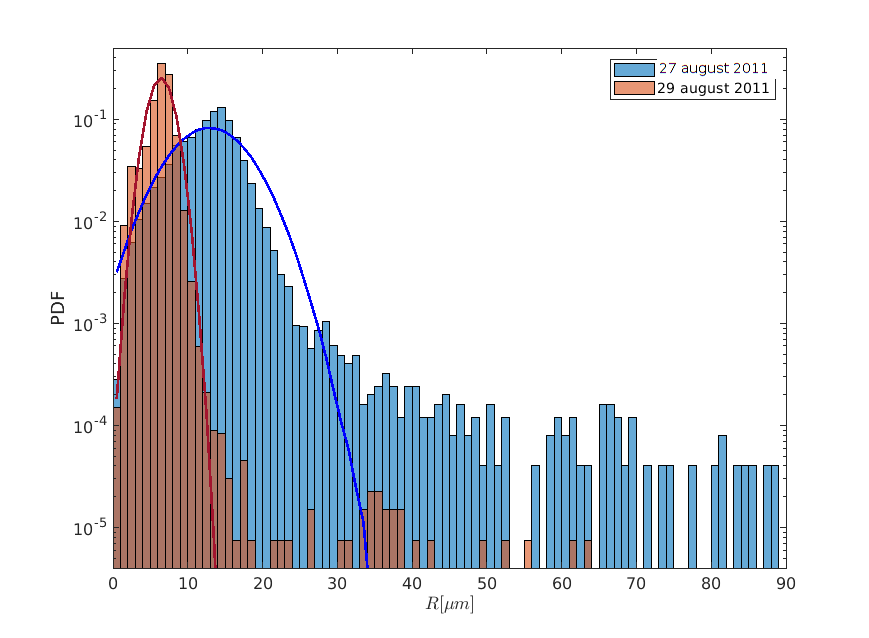
\includegraphics[width=30pc]{PDFs_log.png}
\caption{Droplet size probability distributions calculated for the data obtained with a PDI probe at the UFS on 27th and 29th of August 2011.}
\label{fig:ch4_2}
\end{figure}

Droplet and turbulence measured properties together with derived paremeters are summarized in Table \ref{tab:ch4_1}. The mean values of dimensionless parameters were calculated with the use of mean radius.

\begin{table}
\small
\tabcolsep=0.2cm
\caption{Properties of turbulence and cloud droplets during observation periods.}
\centering
\begin{tabular}{|l|c|c|}
\hline
  & August 27th & August 29th\\
\hline
 Energy dissipation rate $\epsilon$ [m$^2$/s$^3$] & 0.055 & 0.070 \\
\hline
 Kolmogorov length scale $\eta$ [mm] & 0.50  & 0.47\\
\hline
Komogorov timescale $\tau_{\eta}$ [s] & 0.017 & 0.015\\
\hline
 Mean droplet radius $R$ [$\mu$m] & 12.9 $\pm$ 4.8 & 6.4 $\pm$ 1.5\\
\hline
 Stokes number $St$ (mean) & 0.126  & 0.035\\
\hline
 Sedimentation parameter $Sv$ & 0.676  & 0.172\\
 \hline
 Froude number $Fr$ & 0.431  & 0.470\\
 \hline
 Number density $n$ [cm$^{-3}$] & 56 $\pm$ 47 & no data\\
 \hline
%\multicolumn{2}{l}{$^{a}$Footnote text here.}
\end{tabular}
\label{tab:ch4_1}
\end{table}

\begin{figure}[h]
\centering
\noindent\includegraphics[width=35pc]{fig01.png}
\caption{Examples of cloud voids observed at the UFS station with various camera-laser configurations. Images taken on 27 August (panel a) were chosen to estimate cloud void sizes. The ones recorded on 29 August evening (panel b) show the difference between inhomogeneities produced by cloud voids and those resulting from the mixing with clear air at the cloud edge. Other images from 29 August (panel c) suggest that the voids can be quite frequent in the sample volume. Bright spots and lines are due to presence of larger precipitation particles. 10~cm long segment is shown to represent spatial scale assumed in the void size calculation. For more details, see the movies attached in the supplementary materials.}
\label{fig:ch4_3}
\end{figure}

Two kinds of events in which droplet spatial distribution is visibly inhomogeneous were distinguished in the collected images. The first kind was characterized by an irregular interface separating clear-air and cloudy-air volumes and/or cloudy volumes of visibly different properties over a wide range of spatial scales (panel b) in Fig. \ref{fig01}). Inhomogeneities of the second kind, present within the cloudy volumes, were called cloud voids in ``Swiss cheese" clouds. Cloud voids were small (a few centimeters scale), the interface was usually blurry (see panels a) and c) in Fig. \ref{fig01}) and the shapes of clear-air regions were often close to round or elliptic (see magnified voids in Fig. \ref{fig03}). It is important to point out that the more intuitive expression "cloud holes" with regards to these inhomogeneities is avoided on purpose because it is commonly used referring to the cloud-free regions occurring in stratocumulus decks, as described for example in \citet{Gerber_2005}. Inhomogeneities of the first kind are argued to be created in the process of cloud -- clear-air mixing (e.g. \cite{Warhaft_2000}). In contrast, in some series of images and movies, the shape of the recorded tracks of cloud droplets suggest the following cloud void origin hypothesis: they result from interactions between inertial, heavy cloud droplets and small-scale vortices present in a turbulent cloud. Comparison of the two described cases becomes straightforward when conducted on the basis of the movies in the database \citep{database}. In the movie "ms01" between 13~s and 22~s there are two cloud void appearances. Motion of the void in the homogeneous cloud field resembles motion of a worm. Movie "ms02" presents cloudy and clear air mixing at the cloud edges. \\

\begin{figure}[h]
\centering
\noindent\includegraphics[width=35pc]{fig03.png}
\caption{Example close-ups of variously shaped cloud voids observed at the UFS station with different camera-laser configurations. 5~cm long segment is shown to represent spatial scale assumed in the void size calculation.}
\label{fig03}
\end{figure}

There were a few series of cloud void images collected with various laser-camera settings on the two experimental days. The best quality series, made in the morning of the 27th, was chosen for void size analysis. For the series of 17 photos selected for analysis, there were four in which voids were not clear enough to be accounted for. In the remaining 13 photos 27 voids were identified. Each one's size was manually determined. In the case of a round void, the diameter was taken as the size; in a case of flattened or ellipsoidal void, the maximal chord was taken. The typical void diameter was estimated to be 3.5$\pm$1~cm; the maximal, 12$\pm$4~cm; the minimal, 1$\pm$0.5~cm. Images from the analyzed series from the morning of August 27th showing examples of objects identified as voids are presented in the panel a) of Fig. \ref{fig01}. Voids captured on the 29th of August were not analyzed due to the large uncertainty resulting from the unknown geometry of the camera-laser set-up. The general experimental observation was that the voids were smaller then those on August 27th. Definitive experimental verification of the cloud void origin is not possible on the basis of collected data only; however, in next sections, we argue that void creation due to inertia of droplets present inside vortex tubes is highly probable.

%------------------------------------------------

\section{Polydisperse particle motion analysis}

Content
%------------------------------------------------
\section{Cloud voids creation mechanism}
Content
\section{Cloud voids simulation}

%------------------------------------------------
\end{document}